% 
% Annual Cognitive Science Conference
% Sample LaTeX Paper -- Proceedings Format
% 

% Original : Ashwin Ram (ashwin@cc.gatech.edu)       04/01/1994
% Modified : Johanna Moore (jmoore@cs.pitt.edu)      03/17/1995
% Modified : David Noelle (noelle@ucsd.edu)          03/15/1996
% Modified : Pat Langley (langley@cs.stanford.edu)   01/26/1997
% Latex2e corrections by Ramin Charles Nakisa        01/28/1997 
% Modified : Tina Eliassi-Rad (eliassi@cs.wisc.edu)  01/31/1998
% Modified : Trisha Yannuzzi (trisha@ircs.upenn.edu) 12/28/1999 (in process)
% Modified : Mary Ellen Foster (M.E.Foster@ed.ac.uk) 12/11/2000
% Modified : Ken Forbus                              01/23/2004
% Modified : Eli M. Silk (esilk@pitt.edu)            05/24/2005
% Modified : Niels Taatgen (taatgen@cmu.edu)         10/24/2006
% Modified : David Noelle (dnoelle@ucmerced.edu)     11/19/2014

%% Change "letterpaper" in the following line to "a4paper" if you must.

\documentclass[10pt,letterpaper]{article}

\usepackage{cogsci}
\usepackage{commath}
\usepackage{graphicx}
\usepackage{pslatex}
\usepackage{siunitx}
\usepackage{apacite}
\usepackage{xcolor}  % for \textcolor

\newcommand{\todo}[1]{\textbf{\textsc{\textcolor{blue}{(TODO\@: #1)}}}}

\title{A Spiking Independent Accumulator Model for Winner-Take-All Computation}

\author{{\large \bf Jan Gosmann (jgosmann@uwaterloo.ca)} \\
  {\large \bf Aaron R. Voelker (arvoelke@uwaterloo.ca)} \\
  {\large \bf Chris Eliasmith (celiasmith@uwaterloo.ca)} \\
  Centre for Theoretical Neuroscience, University of Waterloo \\
  Waterloo, ON, Canada N2L 3G1
}

\begin{document}

\maketitle

\begin{abstract}  % 150 word limit
Winner-take-all (WTA) mechanisms are an important component of many cognitive models.
For example, they are often used to decide between multiple choices or to selectively direct attention.
Here we compare two biologically plausible, spiking neural WTA mechanisms. 
We first provide a novel spiking implementation of the well-known leaky, competing accumulator (LCA) model, by mapping the dynamics onto a population-level representation.
We then propose a two-layer spiking independent accumulator (IA) model, and compare its performance against the LCA network on a variety of WTA benchmarks.
Our findings suggest that while the LCA network can rapidly adapt to new winners, the IA network is better suited for stable decision making in the presence of noise.

\textbf{Keywords:} Neural Engineering Framework; Nengo; winner-take-all; decision making; mutual inhibition; neural competition; dynamical systems
\end{abstract}

\section{Introduction}
Winner-take-all (WTA) networks are mechanisms that select the largest value among a number of inputs.
More precisely, given a $D$-dimensional vector corresponding to the non-negative utility of $D$ different choices, the desired output is positive for the dimension with highest utility (i.e.,~the ``winner'') and zero for all others.
This mechanism is regularly employed as a component of cognitive models involving selective attention~\cite<e.g.,>{itti1998,standage2005} and decision making, where the action with the highest utility is selected to drive behaviour~\cite<e.g.,>{oreilly1998}.

A large body of literature examines the optimality of WTA mechanisms and their consistency with neurobiological and psychological data~\cite<e.g.,>{bogacz2006,gold2007,smith2004}.
Here, we investigate the suitability of two different WTA mechanisms in the context of neurally plausible cognitive modelling.
In particular, we map each mechanism onto a network of spiking neurons, and then compare them using a set of functional benchmarks that are normative in nature.
The first mechanism we consider is an implementation of the \emph{leaky, competing accumulator} (LCA) model from~\citeA{usher2001}.
The LCA model and variants have been widely used, for example in versions of the Temporal Context Model~\cite{sederberg2008}, and in work on the Remote Associates Test models~\cite<e.g.,>{kajic2017}.
The second mechanism we consider is the \emph{independent accumulator} (IA) model that we propose here, which involves a secondary thresholding layer that is recurrently connected to a primary integrating layer.

To implement each model, we use the Neural Engineering Framework~\cite<NEF;>{eliasmith2003} to map the model's dynamics onto populations of spiking neurons.
In the remainder of the paper, we provide a short introduction to the NEF, describe our implementation of the two WTA mechanisms, present our benchmarks, and finally discuss some resulting implications for cognitive modelling.

\section{Methods}

\subsection{The Neural Engineering Framework}
The Neural Engineering Framework~\cite<NEF;>{eliasmith2003} is a method for mapping a cognitive model, described using mathematical equations, onto a spiking neural network.
We now describe the aspects of this framework that are relevant to this work, by summarizing its three principles: \emph{representation}, \emph{transformation}, and \emph{dynamics}.

\subsubsection{Principle 1: Representation}
We define the representation of a scalar value $x(t)$ by an encoding and decoding with respect to some population of neurons.
The encoding of $x(t)$ into a spike train $a_i(t)$ for neuron $i$ is given by:
\begin{equation}
    a_i(t) = G_i\left[\alpha_i e_i x(t) + J_i^{\mathrm{bias}}\right] ,
\end{equation}
where $\alpha_i$ is a gain factor, $e_i$ is an encoder that determines a neuron's tuning curve, $J_i^{\mathrm{bias}}$ a bias current, and $G_i \left[ \cdot \right]$ is the neural nonlinearity.
Here, we use spiking, leaky integrate-and-fire (LIF) neurons for $G_i \left[ \cdot \right]$, and set the encoders to one.
Decoding weights $d_i$ are then used to approximate the represented value $\hat x(t)$ from the activity of the population of neurons by:
\begin{equation}
    \hat x(t) = \sum_i d_i \left[(a_i * h)(t)\right] ,
\end{equation}
where $h(t) = \tau_{\mathrm{s}}^{-1}\exp(-t/\tau_{\mathrm{s}})$ is an exponentially decaying synaptic filter with time-constant $\tau_{\mathrm{s}}$, and $\ast$ is the convolution operator.
The decoding weights are obtained by least-squares optimization of the error $E_x = \abs{x - \hat{x}}$.
For the transmission of a value from one population to another, the connection weights are given by:
\begin{equation}
    W_{ij} = \alpha_j e_j d_i \text{.}
\end{equation}

\subsubsection{Principle 2: Transformation}
By finding alternate decoding weights $d^f_i$ with the error given by $E_{f(x)} = \abs{f(x) - \hat x}$, arbitrary linear and nonlinear functions $f(x)$ can be approximated in the connections between neural populations.

\subsubsection{Principle 3: Dynamics}
Given some desired nonlinear dynamics for the state variable $x(t)$:
\begin{equation} \label{eqn:nonlinear-system}
    \frac{\partial x}{\partial t} = g(x) ,
\end{equation}
we can map these dynamics onto a recurrent transformation, by harnessing the synaptic filter mentioned in Principle 1.
In particular, for the exponentially decaying $h(t)$ we may apply Principle 2 to the recurrent transformation $f(x) = \tau_s g(x) + x$ to ensure that $x(t)$ obeys Equation~\ref{eqn:nonlinear-system}.

\subsection{Leaky, competing accumulator model}
Using the principles of the NEF, we have implemented the widely-used leaky, competing accumulator (LCA) model proposed by~\citeA{usher2001}.
The dynamics (see Fig.~\ref{fig:usher-mcclelland}a) for each state variable $x_i(t),\ 1 \leq i \leq D$, where $D$ is the number of choices, are given by:
\begin{equation} \label{eqn:usher-mcclelland}
    \begin{split}
        \frac{{\partial x}_i}{\partial t} = \left(\rho_i - kx_i - \beta \sum_{j \neq i} x_j\right) \frac{1}{\tau}, \quad x_i &\ge 0,
    \end{split}
\end{equation}
where $\rho_i$ is each external input, $k$ is the leak rate, $\beta$ the lateral inhibition, and $\tau$ the integration time-constant.
This model essentially integrates each input $\rho_i$ with a leak term ($- kx_i$), minus competition from every other variable ($\beta \sum_{j \neq i} x_j$).
Supposing $\rho_i > \rho_j$ for all $j \ne i$, a WTA mechanism should indicate that $i$ is the winning choice.
Setting $k = \beta = 1$ will guarantee that the winning state $x_i$ converges to the value of the largest input $\rho_i$, while each losing state $x_j$ ($j \ne i$) converges to zero.
Other choices of $k$ merely alter the effective $\tau$ and the effective gain on the input, while other choices of $\beta$ will produce unwanted behaviours (see supplementary analysis).

We implement Equation~\ref{eqn:usher-mcclelland} with the NEF by using one population of neurons for each $x_i$, and applying Principle~3 to each population.
By appropriately selecting the gain and bias parameters from Principle~1, we ensure that each state variable is rectified ($x_i \ge 0$) as required.
We believe this implementation is novel as it does not interpret each $x_i$ as a distinct neural firing rate, but rather as a population-level representation distributed across any number of spiking neurons.
In effect, heterogeneous spike trains are weighted by optimal decoding weights to precisely implement the stated dynamics.
%As such, the model equations do not impose restrictions on the neuron model or requires to lump the neurons into a single population firing rate.
This allows us to attain greater biological realism without altering the dynamics prescribed by Equation~\ref{eqn:usher-mcclelland}.
\begin{figure}[t]
    \centering
    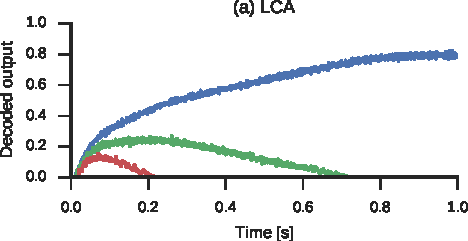
\includegraphics{figures/lca}\\
    \vspace*{.3cm}
    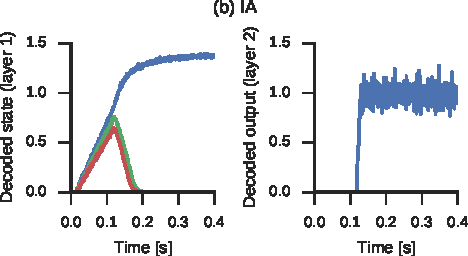
\includegraphics{figures/ia}
    \caption{
        Example time course of the state variables in the LCA (top) and IA (bottom) networks with three choices ($D~=~3$).
        The vector of inputs is $\left[ 0.8, 0.7, 0.6 \right]$.
    }\label{fig:usher-mcclelland}\label{fig:indacc}
\end{figure}

\subsection{Independent accumulator model}
The other WTA mechanism that we investigate is our proposed independent accumulator (IA) model (see Fig.~\ref{fig:ia-sketch}).
We use the term `independent' to refer to the fact that there are no direct interactions between each accumulator, unlike in the LCA model which has direct competition between states.
To enable a form of competition, we add a second thresholding layer that  projects back to self-excite and mutually-inhibit the first layer.
We now provide the details of each layer~-- again implemented using the principles of the NEF\@.
\begin{figure}
    \centering
    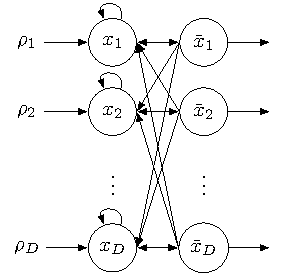
\includegraphics{figures/ia-sketch}
    \caption{
        Independent accumulator (IA) network.
        Neural populations are denoted by circles labelled with their represented state variable.
        Arrows denote excitatory connections, while lines ending in circles denote inhibitory connections.
        The second layer computes $\bar{x}_i := \Theta(x_i - \vartheta)$.
    }\label{fig:ia-sketch}
\end{figure}

The first layer consists of a separate integrator population (i.e., accumulator) for each state variable $x_i(t), \ 1 \leq i \leq D$.
The second layer consists of independent, non-recurrent populations that receive input from the first layer in a one-to-one fashion.
From the second layer, we decode the function $\bar{x}_i := \Theta(x_i - \vartheta)$ where $\Theta$ is the Heaviside function, and $\vartheta = 0.8$ is a fixed threshold value that determines how much evidence needs to be accumulated to produce an output.
The Heaviside decoded output of layer 2 projects back to layer 1 to add $\bar{x}_i - \bar{\beta} \sum_{j \neq i} \bar{x}_j$ to the input of $x_i$.
Since intuitively the largest input will accumulate the fastest, once this reaches the threshold $\vartheta$ it will self-excite and inhibit all other state variables.
Fixing $\bar{\beta} = 2$ ensures that the losing state variables will go to zero (see supplementary analysis).
This is summarized more precisely by the following dynamics (see Fig.~\ref{fig:indacc}b):
\begin{equation}
    \begin{split}
        \frac{{\partial x}_i}{\partial t} = \rho_i \frac{1}{\tau_1} + \left( 
            \bar{x}_i - \bar{\beta} \sum_{j \neq i} \bar{x}_j \right) \frac{1}{\tau_2} , \quad x_i &\ge 0 .
    \end{split}
\end{equation}
Notably, this takes the form of Equation~\ref{eqn:usher-mcclelland} after substituting $\tau = \tau_1$, $k = -\tau_1/\tau_2$, and $\beta = \bar{\beta}\tau_1/\tau_2$, with the only remaining difference being the Heaviside nonlinearity applied to the state feedback.
Thus, in contrast to the continual competition occurring in the LCA model, the threshold $\vartheta$ is a free parameter that controls how much evidence needs to be integrated before enabling any competition between states.
Instead of directly manipulating $\vartheta$, we opt to change $\tau_1$, which has a comparable effect due to the leak-free integration.

Note that the layer 2 decoded output of a single choice shows more variance in the IA network (Fig.~\ref{fig:indacc}), but the separation of the output for different choices is more relevant in interpreting the output.

\subsection{Benchmarks}
To test and compare the two WTA mechanisms we provide an input of $\rho_i = u - s(1 - \delta_{1i}) + \eta_i$, where $u$ is the magnitude of the largest input, $s > 0$ is the target separation relative to all other inputs, $\delta$ is the Kronecker delta, and $\eta_i$ is Gaussian (white) noise with standard deviation $\sigma$.
Thus, without loss of generality, the first state variable receives the largest input $u$ plus noise, and all other state variables receive a noisy input that is smaller by $s$.
It is important to note that $u$ not only determines the size of the largest input, but also the general baseline of inputs.
Since all of the runner-ups have equal magnitude, this represents the most difficult scenario for the networks, where all potential choices must be considered.
As $s \rightarrow 0$ the problem also becomes more difficult because the utilities of the choices are closer together.
We use $u = 1$ unless indicated otherwise, and set the number of choices to $D = 10$.
Furthermore, we increment the noise variance to highlight successes and failures as the task becomes increasingly difficult with more noise.
This allows us to determine which functions are performed robustly by each network.
In both WTA models we use 200 neurons per choice.
In the IA network this is split into 150 neurons for each layer 1 population and 50 neurons for each layer 2 population.
All remaining network parameters are summarized in Table~\ref{tbl:params}.
\begin{table}
    \caption{Summary of parameter values.}\label{tbl:params}
    \begin{tabular}{ll}
        LCA time-constant & $\tau = \SI{0.1}{\second}$ \\
        LCA recurrency parameters & $k = \beta = 1$ \\
        IA accumulation time-constant & $\tau_1 = \SI{0.1}{\second},\ \SI{0.5}{\second}$ \\
        IA feedback time-constant & $\tau_2 = \SI{0.1}{\second}$ \\
        IA threshold & $\vartheta = 0.8$ \\
        IA recurrency parameters & $\bar{\beta} = 2$ \\
        Recurrent synaptic time-constant & $\tau_{\mathrm{s}} 
        = \SI{0.1}{\second}$ \\
        Feed-forward synaptic time-constant & $\tau_{\mathrm{s}} 
        = \SI{0.005}{\second}$ \\
        Output decoding synaptic time-constant & $\tau_{\mathrm{s}} 
        = \SI{0.01}{\second}$
    \end{tabular}
\end{table}

To evaluate the two mechanisms on the previously defined input, we use a number of separate metrics.
First, we determine whether the model is able to form a clear decision within one second.
To be counted as `clear', at least one output must remain above 0.15 across the time interval $(\SI{1}{\second}, \SI{2}{\second}]$ while all other outputs remain below this threshold. % chktex 9
This lower bound of 0.15 was chosen to ensure that noise on a zero output is not mistaken for a non-zero output.
Note that this metric requires that the decision does not change throughout the time interval.
This does not take into account whether the winning output actually corresponds to the largest input. 
However, for some models it is more desirable to produce a clear incorrect decision than an unstable incorrect decision.
In other situations, though, the correctness of the decision may be of higher importance.
Thus, we consider a trial `correct' if the model forms a clear decision, and the largest output corresponds to the true largest input.  
Measurement of correct trials forms our second benchmark.

We use two additional benchmarks on the set of all trials with a clear decision.
First, it is important to consider the speed at which the network can make decisions.
We therefore define the `decision time' as the length of time it takes to fulfil the conditions of a clear decision.
Second, the correctness metric only considers the final averaged output during a time interval.
It is possible for a network to produce transient outputs before the final decision is reached.
In the context of a larger model, this can become a problem because the transient output might be prematurely interpreted as a decision.
Thus, we define it as the `highest output of a losing choice' during the whole simulation.

\section{Results}
We find that the ability to form a clear decision of the LCA network decreases with more noise and less target separation  (see Fig.~\ref{fig:decisions}).
Also, the magnitude of the inputs has an important influence.
For a small inputs with $u=0.2$ the winner will mostly not exceed the 0.15 threshold with noise present.
The best performance is achieved with medium inputs with $u=0.6$.
Higher inputs make it more likely that runner-ups will exceed the 0.15 threshold, especially with a small target separation.
In contrast to the LCA network, the IA network manages to form a clear decision in every trial (not explicitly shown in Figure~\ref{fig:decisions}, but all data points fall on the grey line).
\begin{figure*}[t]
    \centering
    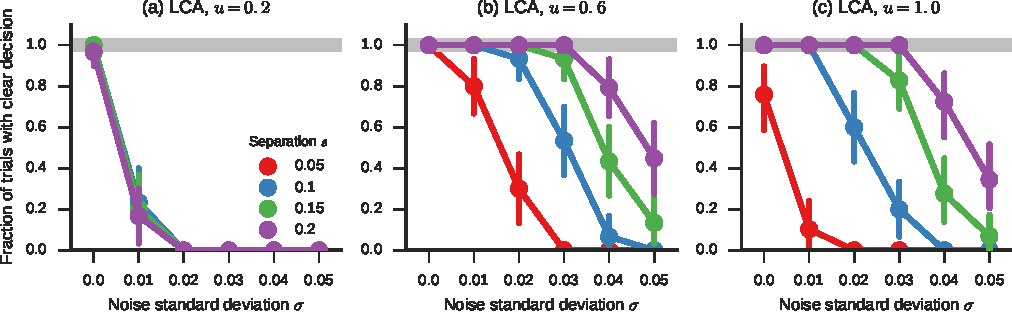
\includegraphics{figures/decisions}
    \caption{
        Fraction of trials with a clear decision for the LCA network (which also exactly matches the fraction of correct trials).
        Each plot shows data for a different input magnitude $u$.
        Error bars denote bootstrapped 95\% confidence intervals.
        The grey horizontal line indicates the optimum, which coincides with the performance of the IA network.
    }\label{fig:decisions}
\end{figure*}

Interestingly, for all clear decisions the correct winner was determined by the LCA network.
Thus, a plot of correct trials looks identical to Figure~\ref{fig:decisions}, with slightly different error bars.
While always reaching a clear decision, the decisions of the IA network are not always correct.
Overall, the IA performance tends to be worse than the LCA performance for a high input magnitude, but better for smaller inputs (Fig.~\ref{fig:correct}a,\,b).
We can greatly improve the IA performance by increasing $\tau_1$ to \SI{0.5}{\second} which slows down the integration of evidence (Fig.~\ref{fig:correct}c).
This improves the IA performance to be above the LCA performance for high baselines, but it will also increase the decisions times of the IA network.
For a low baseline with $u=0.2$, it makes the IA network unable to decide within the allocated time frame, but given more time it would still reach a decision.
%A further improvement to the IA network is possible by eliminating a systematic bias introduced in the second layer of the IA network.
%In the NEF the neuron gain and bias parameters are usually picked from random distributions.
%As such the layer 2 populations will become active at slightly different thresholds.
%By using identical layer 2 populations, i.e., identical gain and bias parameters for each population, this bias can be eliminated and the IA network performs even better (Fig.~\ref{fig:correct}d).
\begin{figure*}[t]
    \centering
    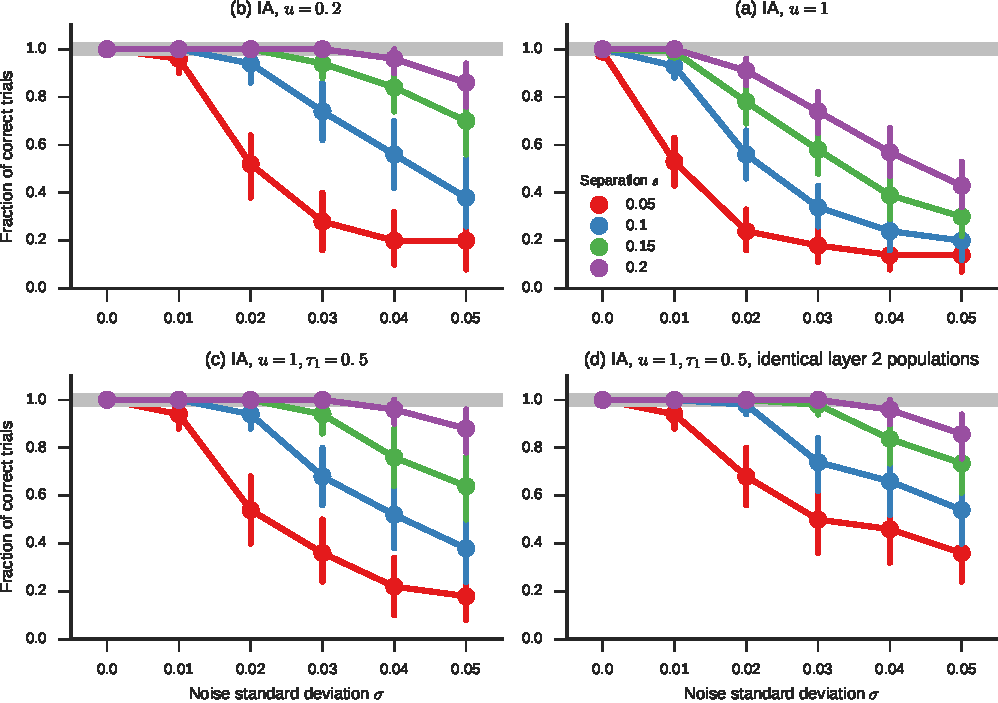
\includegraphics{figures/correct}
    \caption{
        Fraction of correct trials for the IA network.
        Each plot shows data for a different combination of input magnitude $u$ and integration time-constant $\tau_1$.
        Error bars denote bootstrapped 95\% confidence intervals.
        The grey horizontal line indicates the optimum.
    }\label{fig:correct}
\end{figure*}

As shown in Fig.~\ref{fig:time}a, the time required to reach a decision in the LCA network depends mostly on the size of inputs and target separation.
We averaged over the different noise conditions because the noise influence on the timing was minor.
In the IA network the largest input is the most important factor (dashed vs.\ solid lines in Fig.~\ref{fig:time}b).
Depending on this magnitude, the network can either be faster or slower than the LCA network, but it will need more time given a value of $\tau_1$ that achieves the same fraction of correct responses as the LCA network.
There is also a slight influence of target separation and input noise, with an interaction of these two parameters (solid lines in Fig.~\ref{fig:time}).
\begin{figure*}[t]
    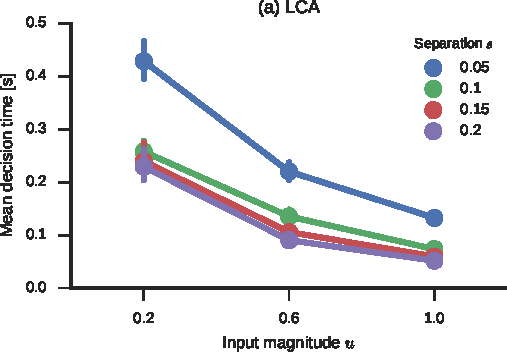
\includegraphics{figures/time1}
    \hfill
    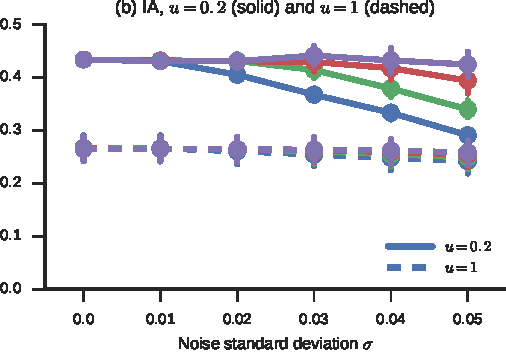
\includegraphics{figures/time2}
    \caption{
        (Left) Mean decision times for the LCA network.
        Shown data is averaged across all noise levels, since noise had minimal effect on decision times.
        (Right) Mean decision times for the IA network with input magnitude $u = 0.2$ (solid) and $u = 1$ (dashed).
        Error bars denote bootstrapped 95\% confidence intervals.
    }\label{fig:time}
\end{figure*}


Finally, looking at the transient responses indicates that both models might produce outputs of losing choices.
For the LCA network the magnitude of the transient response mainly increases with the amount of noise (Fig.~\ref{fig:transient}a).
For the IA network, transient outputs are smaller in noisy conditions, but can be higher than for the LCA network in less noisy conditions with small target separations.
The magnitude of such transient responses is reduced by adjusting $\tau_1$ to 0.5, at the cost of a slower decision.
\begin{figure*}
    \centering
    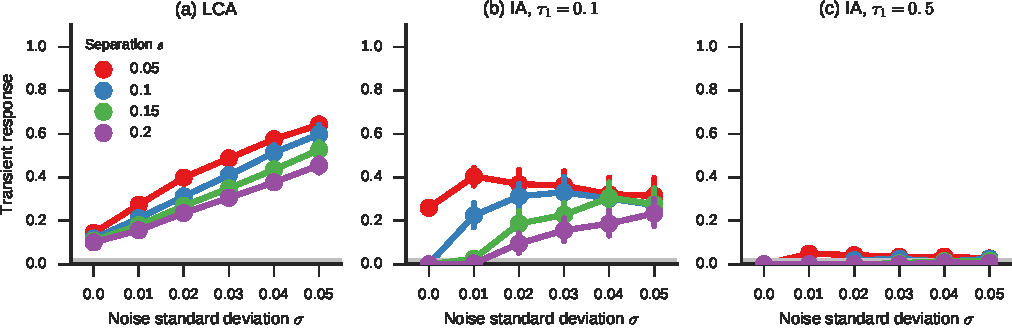
\includegraphics{figures/transient}
    \caption{
        Transient response (highest output of losing choices) for the LCA and IA network.
        Error bars denote bootstrapped 95\% confidence intervals.
        The grey horizontal lines show the optimum.
    }\label{fig:transient}
\end{figure*}

\section{Discussion}
We have shown that neither network performs better on all benchmarks, but rather each is better suited for different purposes.
For instance, the LCA network can determine the correct winner more quickly, and, given that a conclusive decision was made, it always selects the correct winner.
However, under noisy conditions it may fail to produce a clear output at all, and thus not make a decision.
This can be problematic for cognitive models that must form a clear decision (even when it may be incorrect).
The IA network might not be able to identify the correct winner as quickly or as reliably (depending on the choice of $\tau_1$), but given enough time it will eventually arrive at a decision and produce a clear output.
This is a direct consequence of the thresholding on the state feedback, which prevents competition from occurring until a sufficient amount of evidence has accumulated.
This also enables the IA network to react to small inputs.
In addition, the IA network is easily extendible to allow dynamic control of the decision speed, by supplying an external bias to layer 2 to adjust the $\vartheta$ threshold.

The LCA network is especially well-suited for situations where a decision needs to be continuously adjusted.
The dynamics constantly push the winning state variable to the magnitude of the largest input, while adapting to input changes along a time-scale of $\tau$.
This makes it quick to respond to changes in the input for smaller $\tau$, but leads to randomly switching outputs due to noise.

In contrast, the IA network is better suited for situations where a discrete sequence of decisions is required.
After selecting a winner, the model's decision will persist due to self-excitation, even in the absence of input.
Thus, after making a decision, it is necessary to reset the model by inhibiting the winning accumulator.
This limits how quickly successive decisions can be made and reduces the ability to react to changing inputs.
However, once a decision is made, the network provides a stable output.
As an example, we intend to use the IA network in a free recall memory model where a clear response needs to be selected.
A non-correct response in this case might still be a valid response in the context of this task and could be better than no response at all.

Both models might produce a transient response that may be interpreted as a decision, which can make the detection of decisions problematic.
This is of special relevance when incorporating the networks into larger cognitive models.
For the LCA network, the transient behaviour is inherent to its design; there will always be an initial rise of all state variables (that receive input) before the mutual inhibition grows strong enough to push them back to zero.
In the IA network, however, such transient responses may be avoided by choosing appropriate $\tau_1$ and $\vartheta$.
It should be noted that other recurrently connected readout mechanisms with pooled inhibition have been proposed for at least the two choice case~\cite<e.g.>{lo2006} that produce outputs somewhat comparable to the IA network.

%Part of the reason why the IA network produces less correct responses is the systematic bias introduced in the second layer.
%By eliminating this bias through identical ensembles the correctness of the model is increased considerably.
%However, this would require a very precise tuning of the neurons that might not be biologically plausible.


We have not yet investigated the agreement of these mechanisms with neurobiological and behavioural data, although this has been done before for other WTA networks~\cite{gold2007,smith2004}.
The implementation in spiking neurons, however, provides some basic biological plausibility and more readily permits comparisons with neural data.
In particular, the IA network predicts that the firing rates for neurons in the first layer will rise up to a threshold, and that neurons in the second layer will not become active or inhibit the first layer until reaching this threshold.
In contrast, the LCA network predicts that the firing of any neurons will proportionately inhibit all other neurons that do not represent the same state.
With regard to behavioural data, different effects for decision times are predicted as the number of choices increases:
for the LCA network decisions become slower due to the mutual interaction, but for the IA network decisions will take less time because only a single accumulator needs to exceed the threshold.
Nevertheless, evidence for one network does not exclude the possibility that the other network is employed for different tasks or by different brain areas.
Relatedly, it might be more plausible to distribute the representation of all state variables over a single population of neurons.
This is directly supported by the NEF, but we chose to leave this to future work to keep the current analysis free from potential interactions of the state variables introduced by such a distributed representation.

We also did not look at at the influence of the number of dimensions $D$ in detail.
For higher $D$, we see reduced accuracy overall since each additional choice has a baseline chance to win due to noise.
Nevertheless, the results that we discuss here are qualitatively similar.
% With the specific case of only two choices ($D=2$) the decision problem becomes fundamentally easier, since the sum of losing inputs is guaranteed to be below the magnitude of the winner.
% As this case is less general we did not consider it here.

One critique of non-leaky accumulator models is that their ability to discriminate the largest input increases indefinitely with time~\cite{usher2001} and that there is no sensible stopping criterion.
However, this assumes that the time to reach a decision has no cost.
If time-to-decision has a cost, then it will at some point exceed the gain achieved from making a correct decision.
Furthermore, this argument assumes integration with perfect accuracy.
But, with networks built using the NEF, the representation of each state variable has limited precision, and so an ideal trade-off must be found.

To conclude, we investigated two spiking neural networks computing a winner-take-all function based on the leaky, competing accumulator model and a novel two-layer independent accumulator model.
While both perform the same basic tasks, they fail in different ways as each task scales in difficulty via increased noise or less separation between choices.
From a modelling perspective, this makes each network more useful for different situations.
The LCA model is better for continuous updating of decisions, whereas the IA network is better suited for more discrete decisions in the presence of noise.
It is left to future work to investigate whether these two distinct mechanisms can be identified from either behavioural or neurophysiological data.

\section{Notes}
Source code and supplementary analysis are available at \url{https://github.com/ctn-waterloo/cogsci17-decide}.
%These have not been peer reviewed.

\section{Acknowledgments}
This work was supported by the Canada Research Chairs program,
the NSERC Discovery grant 261453, Air Force Office of Scientific Research grant FA8655-13-1-3084, CFI, OIT, and NSERC CGS-D\@.  % chktex 8

\bibliographystyle{apacite}

\setlength{\bibleftmargin}{.125in}
\setlength{\bibindent}{-\bibleftmargin}

\bibliography{references}


\end{document} % chktex 17
